\chapter{Modern GUI Design with Cyberpunk Aesthetics}

This chapter covers the design and implementation of the Smart Relay graphical user interface, built with Rust's \texttt{egui} framework. We explore how to create a modern, AI-assisted interface that simplifies complex networking operations while maintaining a distinctive cyberpunk visual identity.

\section{Design Philosophy}

The GUI is designed with several key principles:

\begin{itemize}
    \item \textbf{Simplicity through AI}: Complex configuration is abstracted away by AI-driven recommendations
    \item \textbf{Visual Feedback}: Real-time status indicators and health monitoring
    \item \textbf{Cross-Platform}: Native performance on Windows, macOS, and Linux
    \item \textbf{Cyberpunk Aesthetic}: Dark themes with neon accents for a distinctive look
\end{itemize}

\section{Architecture Overview}

The GUI communicates with the control plane via HTTP REST API, allowing separation of concerns:

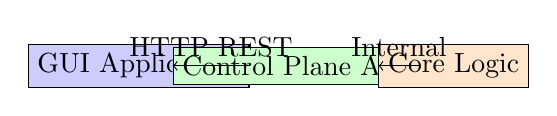
\begin{tikzpicture}[node distance=2cm, auto]
    \node[draw, rectangle, fill=blue!20] (gui) {GUI Application};
    \node[draw, rectangle, fill=green!20, right of=gui] (api) {Control Plane API};
    \node[draw, rectangle, fill=orange!20, right of=api] (core) {Core Logic};
    
    \draw[->] (gui) -- node[above] {HTTP REST} (api);
    \draw[->] (api) -- node[above] {Internal} (core);
\end{tikzpicture}

\section{egui Framework}

\texttt{egui} (immediate mode GUI) provides:

\begin{itemize}
    \item Cross-platform rendering (OpenGL via \texttt{glow} or \texttt{wgpu})
    \item Immediate mode: no retained widget state
    \item Built-in widgets: buttons, text inputs, tables, etc.
    \item Customizable theming
\end{itemize}

\section{Theme Implementation}

The cyberpunk theme uses a dark palette with neon accents and \textbf{white text for optimal contrast}:

\begin{verbatim}
Background:    #0b0f1a (dark navy)
Primary Accent: #00f0ff (cyan)
Secondary:     #ff6bd6 (pink)
Warning:       #ffc800 (amber)
Text:          WHITE (for maximum contrast on dark background)
\end{verbatim}

All text elements use white color to ensure readability against the dark background, with colored accents used only for highlights and status indicators.

\section{Key UI Components}

\subsection{Overview Tab}

The main dashboard showing:
\begin{itemize}
    \item \textbf{Current Connection}: Real-time status, latency, bandwidth usage
    \item \textbf{Quick Stats}: Total endpoints, active connections, subscription count
    \item Connection controls (connect/disconnect)
\end{itemize}

\subsection{Endpoints Tab}

Comprehensive endpoint management with advanced features:

\begin{itemize}
    \item Visual table with enable/disable toggles
    \item Endpoint details: name, host, port, protocol
    \item \textbf{Latency display}: Color-coded latency indicators
    \begin{itemize}
        \item Green: < 100ms (excellent)
        \item Yellow: 100-300ms (good)
        \item Red: > 300ms (poor)
    \end{itemize}
    \item \textbf{Connection status}: Visual highlight for connected endpoints
    \item \textbf{Actions}: Connect, Disconnect, Test, Edit, Delete
    \item \textbf{Right-click context menu}: Batch operations and quick actions
    \item Add/Edit dialog with protocol selection (VMess, VLESS, Shadowsocks, Trojan, SOCKS5)
\end{itemize}

\subsubsection{Right-Click Context Menu}

A sophisticated context menu provides quick access to common operations:

\begin{itemize}
    \item \textbf{Test Connection}: Single endpoint latency test
    \item \textbf{Test All Selected}: Batch test all enabled endpoints concurrently
    \item \textbf{Connect/Disconnect}: Quick connection toggle
    \item \textbf{Edit}: Modify endpoint configuration
    \item \textbf{Delete}: Remove endpoint (with confirmation)
    \item \textbf{Copy URL}: Copy endpoint URL to clipboard (future)
\end{itemize}

Implementation uses \texttt{egui::Window} with fixed positioning at the click location.

\subsection{Subscriptions Tab}

Subscription import and management:
\begin{itemize}
    \item Import from URL or file
    \item Subscription list with update timestamps
    \item Endpoint count per subscription
    \item Update and delete operations
\end{itemize}

\subsection{Configuration Tab}

Client and port configuration with system proxy integration:

\begin{itemize}
    \item \textbf{Port Configuration}: Local port, SOCKS5 port, HTTP port (with validation)
    \item \textbf{Client Parameters}:
    \begin{itemize}
        \item Auto Start on Boot
        \item Start Minimized
        \item Allow LAN Connections
        \item Use Local DNS
    \end{itemize}
    \item \textbf{System Proxy Mode}:
    \begin{itemize}
        \item \textbf{Unchanged}: Don't modify system proxy settings
        \item \textbf{Direct}: Disable system proxy (no proxy)
        \item \textbf{Global}: Route all traffic through proxy
        \item \textbf{PAC}: Use Proxy Auto-Configuration script
    \end{itemize}
    \item \textbf{Proxy Exceptions}: Semicolon-separated list of domains/IPs to bypass
    \item \textbf{Apply Proxy Settings}: Button to apply configuration to Windows system
\end{itemize}

When connecting to an endpoint, if "Apply to System" is enabled, the Windows system proxy is automatically configured according to the selected mode. On disconnect, the proxy is disabled to restore original settings.

\subsection{Xray Settings Tab}

Advanced Xray core configuration:
\begin{itemize}
    \item Log level (Debug, Info, Warning, Error)
    \item DNS servers configuration (multi-line)
    \item Routing domain strategy (AsIs, IPIfNonMatch, IPOnDemand)
    \item Traffic sniffing toggle
    \item Packet fragmentation toggle
\end{itemize}

\subsection{AI Assistant Tab}

AI-powered configuration assistance:
\begin{itemize}
    \item Natural language goal input
    \item AI recommendation display
    \item One-click configuration application
    \item Integration with Ollama backend
\end{itemize}

\subsection{Status Bar}

Real-time health monitoring of the control plane with visual indicators:
\begin{itemize}
    \item Cyan pulse: Online and healthy
    \item Pink: Connection error
    \item Yellow: Checking status
    \item Gray: Not connected
\end{itemize}

\section{Async State Management}

Since \texttt{egui} is immediate mode, async operations require careful handling. The critical insight is that \texttt{eframe} runs in a synchronous context, but network operations require a Tokio runtime.

\subsection{Runtime Injection Pattern}

\begin{verbatim}
// In main.rs: Create runtime once
let rt = Arc::new(Runtime::new().expect("Failed to create Tokio runtime"));

eframe::run_native("Smart Relay", options, Box::new(move |_cc| {
    let mut app = App::default();
    app.set_runtime(rt.clone());  // Inject runtime
    Box::new(app)
}));

// In App: Store runtime and use for async operations
pub struct App {
    runtime: Option<Arc<Runtime>>,
    // ... other fields
}

fn test_endpoint(&mut self, idx: usize) {
    let rt = self.runtime.as_ref().unwrap();
    let (tx, rx) = mpsc::channel();
    
    rt.spawn(async move {  // Use rt.spawn, not tokio::spawn
        let result = async_operation().await;
        tx.send(result).unwrap();
    });
    
    // Store receiver for processing in update loop
    self.test_receiver = Some(rx);
}

// In update(): Process messages
if let Some(ref mut rx) = self.test_receiver {
    if let Ok(result) = rx.try_recv() {
        // Update UI state with result
    }
}
\end{verbatim}

\subsection{Channel-Based Communication}

Use \texttt{mpsc::channel} for one-way communication from async tasks to GUI:

\begin{itemize}
    \item \textbf{Sender}: Created in async task, sends results.
    \item \textbf{Receiver}: Stored in App state, checked in \texttt{update()} loop.
    \item \textbf{Non-blocking}: Use \texttt{try\_recv()} to avoid blocking the UI thread.
    \item \textbf{Cleanup}: Remove receiver from state after processing all messages.
\end{itemize}

\section{Packaging for Multi-Platform}

\subsection{Windows}

Use PowerShell script to create release zip:
\begin{verbatim}
.\scripts\package-windows.ps1
\end{verbatim}

Creates: \texttt{smart-relay-windows-x86\_64-v0.1.0.zip}

\subsection{Linux}

Creates tarball with binaries:
\begin{verbatim}
bash scripts/package-linux.sh
\end{verbatim}

For \texttt{.deb} packages, additional tooling required (\texttt{cargo-deb}).

\subsection{macOS}

Creates \texttt{.app} bundle and optionally \texttt{.dmg}:
\begin{verbatim}
bash scripts/package-macos.sh
\end{verbatim}

\section{Font Configuration and Internationalization}

\subsection{Chinese Character Support}

Proper font configuration is essential for displaying Chinese characters in endpoint names. The implementation uses a two-tier approach:

\begin{enumerate}
    \item \textbf{Primary}: \texttt{egui-chinese-font} crate automatically detects and loads system Chinese fonts.
    \item \textbf{Fallback}: Manual loading of Windows system fonts (\texttt{msyh.ttc}, \texttt{simsun.ttc}) if automatic detection fails.
\end{enumerate}

\textbf{Key lesson}: Always test with real Unicode content during development, not just ASCII placeholder text.

\subsection{Font Loading Pattern}

\begin{verbatim}
// In main.rs: Setup fonts once during initialization
use egui_chinese_font::setup_chinese_fonts;

eframe::run_native("Smart Relay", options, Box::new(move |cc| {
    if let Err(e) = setup_chinese_fonts(&cc.egui_ctx) {
        eprintln!("Warning: Failed to load Chinese fonts: {}", e);
    }
    // ... rest of initialization
}));
\end{verbatim}

\section{Best Practices}

\begin{itemize}
    \item \textbf{Keep UI responsive}: Offload heavy work to background tasks using Tokio runtime.
    \item \textbf{Provide clear feedback}: Show loading states, success messages, and detailed error messages.
    \item \textbf{Use consistent visual language}: Colors, spacing, and typography should be consistent throughout.
    \item \textbf{Test on all target platforms}: Windows proxy features only work on Windows.
    \item \textbf{Handle errors gracefully}: Never panic on user input or network errors—show user-friendly messages.
    \item \textbf{Visual indicators}: Use color coding for status (green/yellow/red for latency, connection state).
    \item \textbf{Right-click menus}: Provide context-sensitive actions for power users.
    \item \textbf{Async operations}: Always use channels to communicate between async tasks and GUI thread.
    \item \textbf{Font configuration}: Test with actual Unicode content, not just ASCII.
    \item \textbf{State management}: Use \texttt{Default} trait for struct initialization to reduce boilerplate.
\end{itemize}

\section{Future Enhancements}

\begin{itemize}
    \item Real-time connection graphs and bandwidth visualization
    \item Advanced filtering and search with regex support
    \item Plugin system for custom widgets and protocol handlers
    \item Dark/light theme toggle (currently cyberpunk dark only)
    \item Full internationalization (i18n) with language packs
    \item Endpoint grouping and tagging for organization
    \item Connection history and statistics
    \item Export/import endpoint lists as JSON
    \item Clipboard integration for sharing endpoint URLs
    \item Keyboard shortcuts for power users
    \item Real-time latency monitoring with charts
\end{itemize}

